\documentclass{report}
\usepackage[T1]{fontenc}
\usepackage{color}
\usepackage{amssymb}
\usepackage{mathrsfs}
\usepackage{amsmath}
\usepackage{eurosym}
\usepackage{graphicx}
\usepackage{textcomp}
\usepackage{listings}
\usepackage{epigraph}
\usepackage{longtable}
\usepackage{setspace}
\usepackage[some]{background}
\usepackage{gensymb}
\usepackage{tikz}
\usepackage{tabularx}
\usepackage{geometry}
\usepackage{fancyhdr}
\usepackage[english]{babel}
\definecolor{lightgray}{rgb}{0.95, 0.95, 0.95}
\definecolor{darkgray}{rgb}{0.4, 0.4, 0.4}
\definecolor{editorGray}{rgb}{0.95, 0.95, 0.95}
\definecolor{editorOcher}{rgb}{1, 0.5, 0}
\definecolor{editorGreen}{rgb}{0, 0.5, 0} 
\definecolor{orange}{rgb}{1,0.45,0.13}      
\definecolor{olive}{rgb}{0.17,0.59,0.20}
\definecolor{brown}{rgb}{0.69,0.31,0.31}
\definecolor{purple}{rgb}{0.38,0.18,0.81}
\definecolor{lightblue}{rgb}{0.1,0.57,0.7}
\definecolor{lightred}{rgb}{1,0.4,0.5}

\lstdefinelanguage{CSS}{
  keywords={color,background-image:,margin,padding,font,weight,display,position,top,left,right,bottom,list,style,border,size,white,space,min,width, transition:, transform:, transition-property, transition-duration, transition-timing-function}, 
  sensitive=true,
  morecomment=[l]{//},
  morecomment=[s]{/*}{*/},
  morestring=[b]',
  morestring=[b]",
  alsoletter={:},
  alsodigit={-}
}

\lstdefinelanguage{JavaScript}{
  morekeywords={typeof, new, true, false, catch, function, return, null, catch, switch, var, if, in, while, do, else, case, break},
  morecomment=[s]{/*}{*/},
  morecomment=[l]//,
  morestring=[b]",
  morestring=[b]'
}

\lstdefinelanguage{HTML5}{
  language=html,
  sensitive=true,   
  alsoletter={<>=-},    
  morecomment=[s]{<!-}{-->},
  tag=[s],
  otherkeywords={
  >,
    <!DOCTYPE,
  </html, <html, <head, <title, </title, <style, </style, <link, </head, <meta, />,
    </body, <body,
    </div, <div, </div>, 
    </p, <p, </p>,
    </script, <script,
  <canvas, /canvas>, <svg, <rect, <animateTransform, </rect>, </svg>, <video, <source, <iframe, </iframe>, </video>, <image, </image>, <header, </header, <article, </article
  },
  ndkeywords={
  =,
  charset=, src=, id=, width=, height=, style=, type=, rel=, href=,
  fill=, attributeName=, begin=, dur=, from=, to=, poster=, controls=, x=, y=, repeatCount=, xlink:href=,
  margin:, padding:, background-image:, border:, top:, left:, position:, width:, height:, margin-top:, margin-bottom:, font-size:, line-height:,
  transform:, -moz-transform:, -webkit-transform:,
  animation:, -webkit-animation:,
  transition:,  transition-duration:, transition-property:, transition-timing-function:,
  }
}

\lstdefinelanguage{htmlcssjs} {
  basicstyle={\footnotesize\ttfamily},   
  frame=b,
  xleftmargin={0.75cm},
  numbers=left,
  stepnumber=1,
  firstnumber=1,
  numberfirstline=true, 
  identifierstyle=\color{black},
  keywordstyle=\color{blue}\bfseries,
  ndkeywordstyle=\color{editorGreen}\bfseries,
  stringstyle=\color{editorOcher}\ttfamily,
  commentstyle=\color{brown}\ttfamily,
  language=HTML5,
  alsolanguage=JavaScript,
  alsodigit={.:;},  
  tabsize=2,
  showtabs=false,
  showspaces=false,
  showstringspaces=false,
  extendedchars=true,
  breaklines=true
}\lstdefinelanguage{scala}{
morekeywords={%
abstract,case,catch,class,def,do,else,extends,%
false,final,finally,for,forSome,if,implicit,import,lazy,%
match,new,null,object,override,package,private,protected,%
return,sealed,super,this,throw,trait,true,try,type,%
val,var,while,with,yield},
otherkeywords={=>,<-,<\%,<:,>:,\#,@},
sensitive=true,
morecomment=[l]{//},
morecomment=[n]{/*}{*/},
morestring=[b]",
morestring=[b]',
morestring=[b]"""
}[keywords,comments,strings]

\lstset{
float=hbp,
language=scala,
basicstyle=\ttfamily\small\color{colBasic},
upquote=true,
aboveskip={1.5\baselineskip},
columns=fullflexible,
showstringspaces=false,
extendedchars=true,
breaklines=true,
showtabs=false,
showspaces=false,
frame=trbl, 
tabsize=4,
numbers=left,
breakautoindent=true,
extendedchars=true,
showstringspaces=false,
identifierstyle=\ttfamily,
frameround=ffff,
captionpos=b,
xrightmargin=0cm,
xleftmargin=0cm,
backgroundcolor=\color{colBackground},
keywordstyle=\bf\color{colKeyword},
commentstyle=\color{colComment},
identifierstyle=\color{colIdent}, 
stringstyle=\color{colString},}\definecolor{purple}{rgb}{0.5,0,0.41}
\lstset{
float=hbp,
language=java,
basicstyle=\ttfamily\small\color[rgb]{0.20,0.20,0.20},
upquote=true,
aboveskip={1.5\baselineskip},
columns=fullflexible,
showstringspaces=false,
extendedchars=true,
breaklines=true,
showtabs=false,
showspaces=false,
frame=trbl, 
tabsize=4,
numbers=left,
breakautoindent=true,
extendedchars=true,
showstringspaces=false,
identifierstyle=\ttfamily,
frameround=ffff,
captionpos=b,
xrightmargin=0cm,
xleftmargin=0cm,
identifierstyle=\ttfamily,
keywordstyle=\bf\color[rgb]{0.5,0,0.41},
commentstyle=\color[rgb]{0.25,0.37,0.75},
stringstyle=\color[rgb]{0.16,0,1},}\definecolor{colBasic}{rgb}{0.20,0.20,0.20}
\definecolor{colKeyword}{rgb}{0.5,0,0.41}
\definecolor{colBackground}{rgb}{1,1,1}
\definecolor{colComment}{rgb}{0.25,0.37,0.75}
\definecolor{colString}{rgb}{0.16,0,1}
\definecolor{colIdent}{rgb}{0.20,0.20,0.20}


\begin{document}
\renewcommand{\chaptername}{Part}
\renewcommand{\thechapter}{\Roman{chapter}}


%\usepackage{lmodern}
%\usepackage{xspace}
%\usepackage{hyperref}
%\usepackage{fancyhdr}

% header style
\pagestyle{fancy}
\renewcommand{\headrulewidth}{1pt}
\fancyhead[L]{March $3^{rd}$, 2015}
\fancyhead[R]{\textbf{Reference :} model-checking.test-strategy - Version 2}

% Redefine the plain page style
\fancypagestyle{plain}{%
  \fancyhf{}%
  \renewcommand{\headrulewidth}{1pt}
  \fancyhead[L]{March $3^{rd}$, 2015}
  \fancyhead[R]{\textbf{Reference :} model-checking.test-strategy - Version 2}
  \fancyfoot[C]{\thepage}
}

% title page
\definecolor{sup_strip_color}{rgb}{0.70,0.70,0.70}
\definecolor{inf_strip_color}{rgb}{0.00,0.00,0.00}

\DeclareFixedFont{\bigsf}{T1}{phv}{b}{n}{0.9cm}

\makeatletter                       
\def\printauthor{%                  
    {{\large \@author}}}              
\makeatother

\author{Sofia \textsc{Boutahar} ~\\ David \textsc{Courtinot}}

\begin{titlepage}

\newgeometry{left=1cm,right=4cm,bottom=0cm}
\begin{tikzpicture}[overlay,remember picture]
% the black stripe with the title
\node[
  fill=inf_strip_color,
  anchor=north west,
  text width=\paperwidth,
  text height=2cm,
  text depth=2cm,
  inner xsep=1cm,
  font=\color{white}\bigsf 
  ] 
 at ([yshift=-2.5cm]current page.north west) (blackrect) {Test strategy and results - Version 2};
% the khaki stripe
\path[fill=sup_strip_color] 
  (blackrect.north west) rectangle ++(\paperwidth,2.5cm);
\end{tikzpicture}

\vspace*{4.5cm}

\noindent
\begin{minipage}{0.35\linewidth}
    \begin{flushright}
        \printauthor
    \end{flushright}
\end{minipage} \hspace{15pt}
%
\begin{minipage}{0.02\linewidth}
    \rule{1pt}{175pt}
\end{minipage} \hspace{-10pt}
%
\begin{minipage}{0.6\linewidth}
\vspace{5pt}
\newenvironment{test}{\begin{center}}{\end{center}}
\hspace{10pt}
\begin{minipage}{\linewidth} 
\textbf{Reference :} model-checking.test-strategy ~\\
March $3^{rd}$, 2015
\end{minipage}
\end{minipage}

\vspace{8cm}
\begin{minipage}{0.20\linewidth}
    \begin{flushright}
       
        \begin{tabular}{ll}
	 \textit{Signatures} & \\
			& \textbf{Project manager - Zohour \textsc{Abouakil} :} \\
            & \textbf{Quality responsible - David \textsc{Courtinot} :} \\
            & \textbf{Customers - David \textsc{Doose} - Julien \textsc{Brunel} :} \\
        \end{tabular}
    \end{flushright}
\end{minipage}

\end{titlepage}
\restoregeometry
\tableofcontents
\newgeometry{left=2.1cm,right=2.1cm}
\chapter* {Changelog}
\begin{center}
\begin{tabular}{|c|l|l|}
  \hline
  Version & Date & Change  \\
  \hline
  V2 & March $1^{rd}$  & Added the configuration of the tests \\
  & March $1^{rd}$  & Minor redaction fixes \\
  & March $1^{rd}$  & Added more detailed explanations in all the parts \\
  & March $2^{rd}$  & Added CFG part \\
& March $3^{rd}$  & Added the newest tests for the model checker \\
  \hline
\end{tabular}
\end{center}
\chapter* {Overview}
\paragraph{}
\hspace{4mm}\textnormal{The purpose of a test strategy is to clarify the major tasks and challenges of the test project, define what we want to accomplish and how we are going to achieve it. 
Moreover, it helps us figure out if there are missing requirements in the project and have a clear state of it at any point.
Our project is divided into two parts: The conversion of the AST to the CFG and the model checking using CTL.
The first part can be divided into two subparts : parsing the file generated by the Clang compiler and converting the AST to the CFG.}

\chapter{Testing AST conversion to CFG}

\section{Test strategy}

\subsection{Tools and configuration}

\paragraph{}
\hspace{4mm}\textnormal{In order to partly automate our tests and improve the readbility of the output, our test routines automatically call some external tools with the following settings :}

\vspace{3mm}
\begin{itemize}
\item \textbf{Clang API}, version 3.5, options : \textit{-Xclang -ast-dump -std=c++11 -fsyntax-only -w}\vspace{1mm}
\item the \textbf{dot} command, which is part of GraphViz, version 2.29\vspace{1mm}
\end{itemize}

\paragraph{}
\hspace{4mm}\textnormal{Finally, the code was compiled with the official Scala 2.10 compiler.}

\subsection{Approach}

\paragraph{}
\hspace{4mm}\textnormal{When possible, we tried defining automatic test routines or at least to automate all the steps to get the final output, which may have to be manually checked.
If one of our tests fails, we fix it, running the same test over and over until the output is correct.
In some cases, we consider that the parts of the source code concerned by the fix could have an impact on other functionalities. Thus, we check the fix against the other
tests (that were passed prior to the fix). Tests considered as mutually dependent are reunited in the same folder containing the test input files.}

\section{Testing the parser}

\paragraph{}
\hspace{4mm}\textnormal{As the parser simply translates the AST (produced by Clang) in an in-memory tree data-structure, we simply needed to check that
each node of the original AST was correctly converted and that the structure of our parsed AST was the same as the original one.
This cannot be checked automatically so easily, it requires manual checking. However, the Clang API is automatically called by our test
program which prints the output in a file so that the tester can check the result.}

\begin{center}
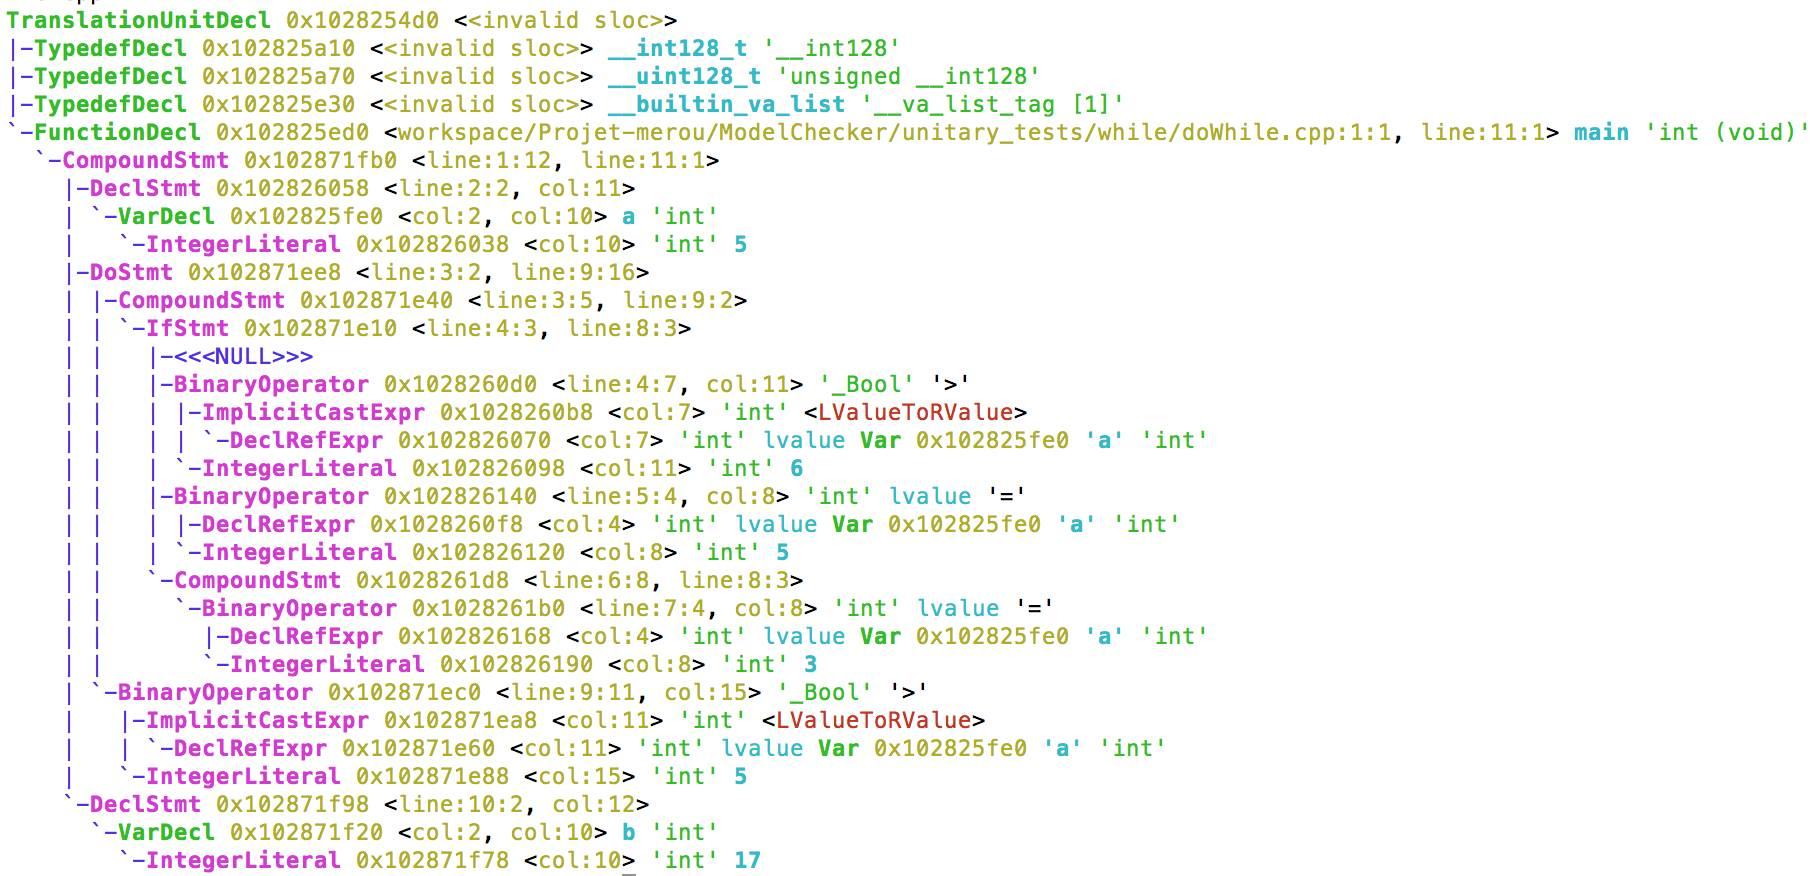
\includegraphics[scale=0.26]{data/dowhile_clang.jpg}
~\\~\\Figure I.1 - Example of an input AST generated automatically of a do-while statement
\end{center}

\begin{center}
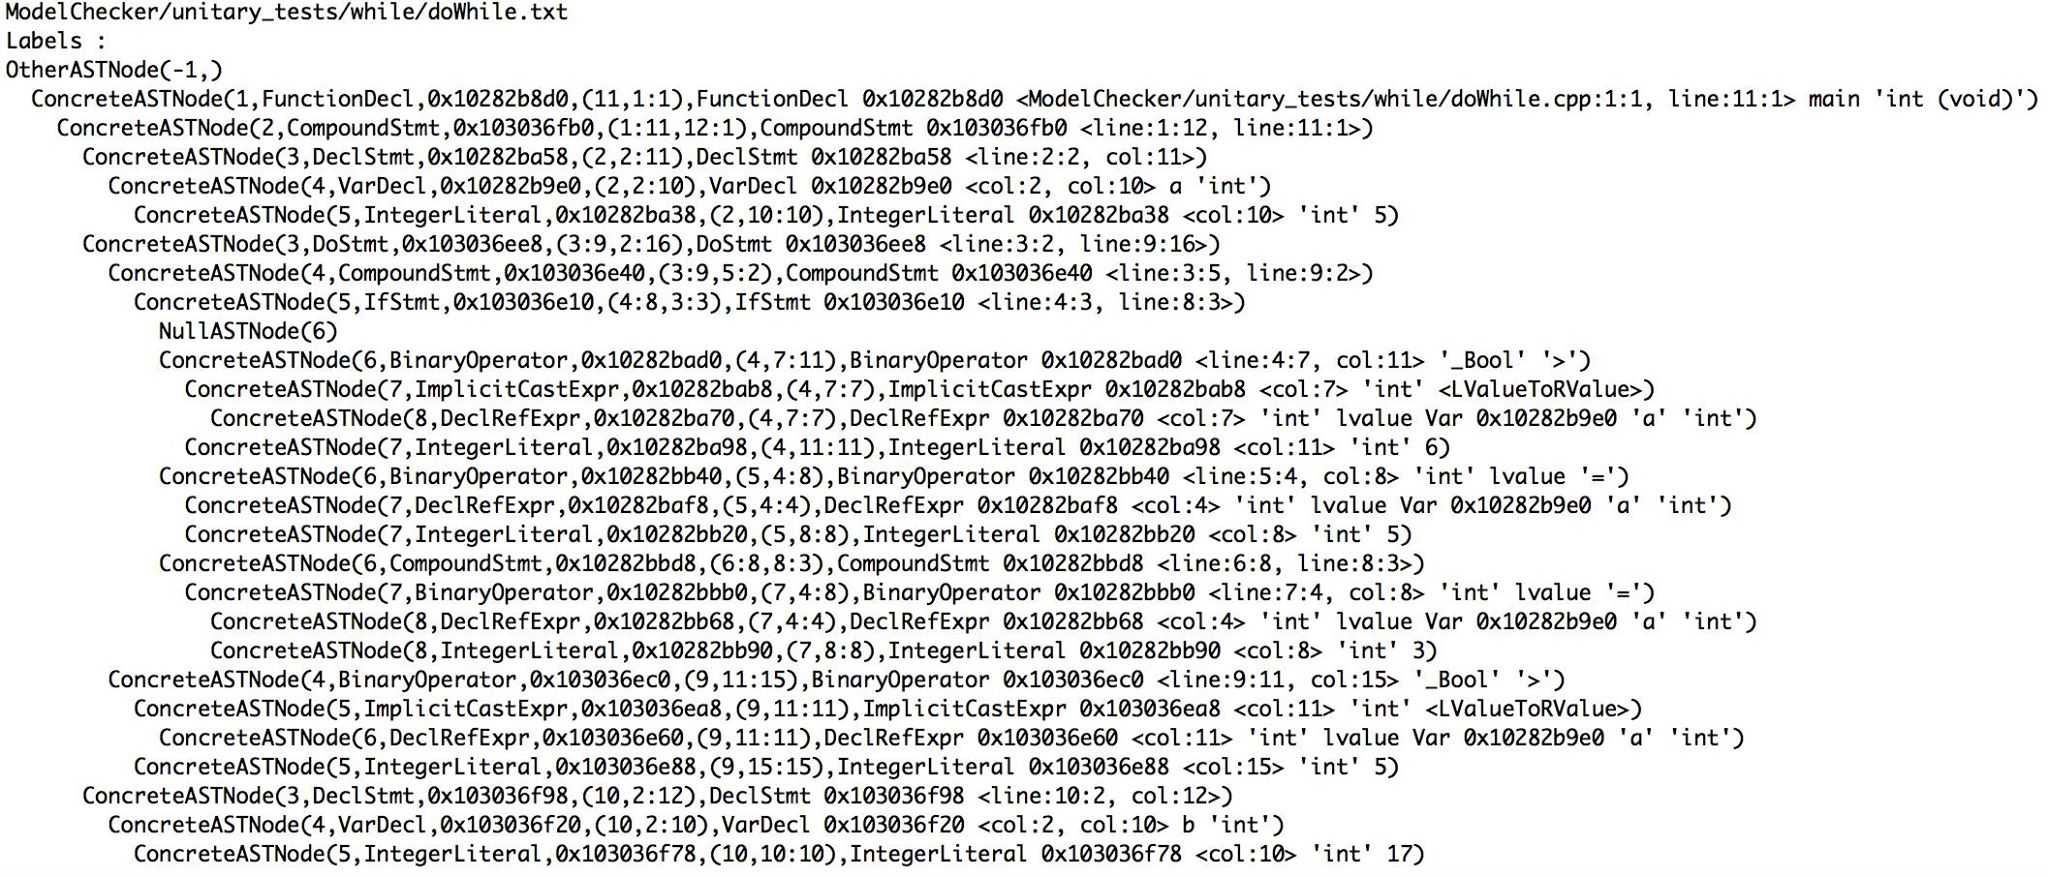
\includegraphics[scale=0.26]{data/while_astNode.jpg}
~\\~\\Figure I.2 - Corresponding output (ASTNode tree data-structure), as the test program prints it
\end{center}

\paragraph{}
\hspace{4mm}\textnormal{The manual checking first consists in comparing the shape of the input and output trees : it must be the same. As you can see it on the above examples,
this is a successful test in this regard. Then, the tester has to verify that all the nodes have been converted to the right kind of node (among ConcreteASTNode,
NullNode and OtherNode) and that the data has been correctly retrieved (line and column of the element in the source code, name of the element, etc).}

\paragraph{}
\hspace{4mm}\textnormal{As the Clang AST treats the same way most kinds of code source element (most of the time, the format is \{ name codePosition args \}), there was no need of unitary tests
strictly speaking, we just ran our test on several examples, starting on small ones to detect minor mistakes and then more complicated ones in the hope that somewhere
in the mass of data we would see an unexpected edge-case.}

\section{Testing the conversion to CFG}

\subsection{Partly automated test}

\paragraph{}
\hspace{4mm}\textnormal{The conversion consists in two steps :}

\vspace{3mm}
\begin{itemize}
\item conversion to an intermediate tree data-structure : SourceCodeNode\vspace{1mm}
\item conversion from SourceCodeNode to the actual CFG\vspace{1mm}
\end{itemize}

\paragraph{}
\hspace{4mm}\textnormal{We decided not writing specific tests for the first step, as it is quite an simple one. Plus, it is uneasy to
validate the output automatically. The second step also requires manual check , however the graph nature of the CFG allowed us to use dot to generate nice graph images
corresponding to our computed CFG. It made it easier to check (visually and quickly) the output of the converter.
To sum up, here is what our test routine does :}

\vspace{3mm}
\begin{itemize}
\item taking a folder path as an input, it calls the Clang API on every cpp file in this folder\vspace{1mm}
\item parses each generated AST\vspace{1mm}
\item convert to SourceCodeNode\vspace{1mm}
\item convert to CFG (the actual implementation type being 	GraphNode[ProgramNode])\vspace{1mm}
\item print the CFG in dot format (text file)\vspace{1mm}
\item call the dot command to generate an image representing the graph\vspace{1mm}
\end{itemize}

\paragraph{}
\hspace{4mm}\textnormal{Generating a graphic output has been a real time saver for us compared to debugging with a textual output as it enabled
us to test highly complex examples without getting confused by the mass of data. It is also important to say that
the way we printed the nodes was indactive of the behaviour of the first step of the conversion. Indeed, the content of the nodes
tells us if the first step went well, and the links in the graph inform us on the second step.}

\subsection{Test cases}

\paragraph{}
\hspace{4mm}\textnormal{Contrarily to the parsing, the conversion to CFG implies very specific processing for different kinds of nodes,
which justifies the fact of writing unitary tests for each kind of node. As an example, here are the input C++ code we used for testing the \textit{for} loop 
(the content is presented in one chunk, but it was actually in separate files to keep the graph clear) :}

\begin{lstlisting}[language=java]
// in all files 
int f() {
    return 3;
}
//////////   Example 1   //////////
int main(int argc, char** argv) {
    int j = 5 + f();
    if (j == 6);
    for (;;);
    int z = 22;
    if ((z-20)==19);
    f();
}
//////////   Example 2   //////////
int main(int argc, char** argv) {
    int j = 5 + f();
    for ( ; 5 < 3 ; );
    f();
}
//////////   Example 3   //////////
int main(int argc, char** argv) {
    f();
    for (int i=3 ; 5 < i ; i++)
        break;
    f();
}
//////////   Example 4   //////////
int main(int argc, char** argv) {
    int j = 5 + f();
    for (int i=3 ; 5 < i ; )
        i -= 5.0;
    f();
}
//////////   Example 5  //////////
int main(int argc, char** argv) {
    int j = f();
    for (int i=3 ; i<5 ; i++)
        i *= 2;
    f();
}
// and so on
\end{lstlisting}
\paragraph{}
\hspace{4mm}\textnormal{As you can see, we try to cover all the possible cases. We did exactly the same with the other elements (\textit{if, while, switch...}).
Then, we tried more complicated things to see if all continued to go well when different kinds of node were mixed. When we detected a bug,
we first identified which nodes were incorrectly rendered, fixed the problem by testing on the complicated example which revealed the issue, and finally
test the fix against the coorresponding unitary tests for non-regression.}

\begin{center}
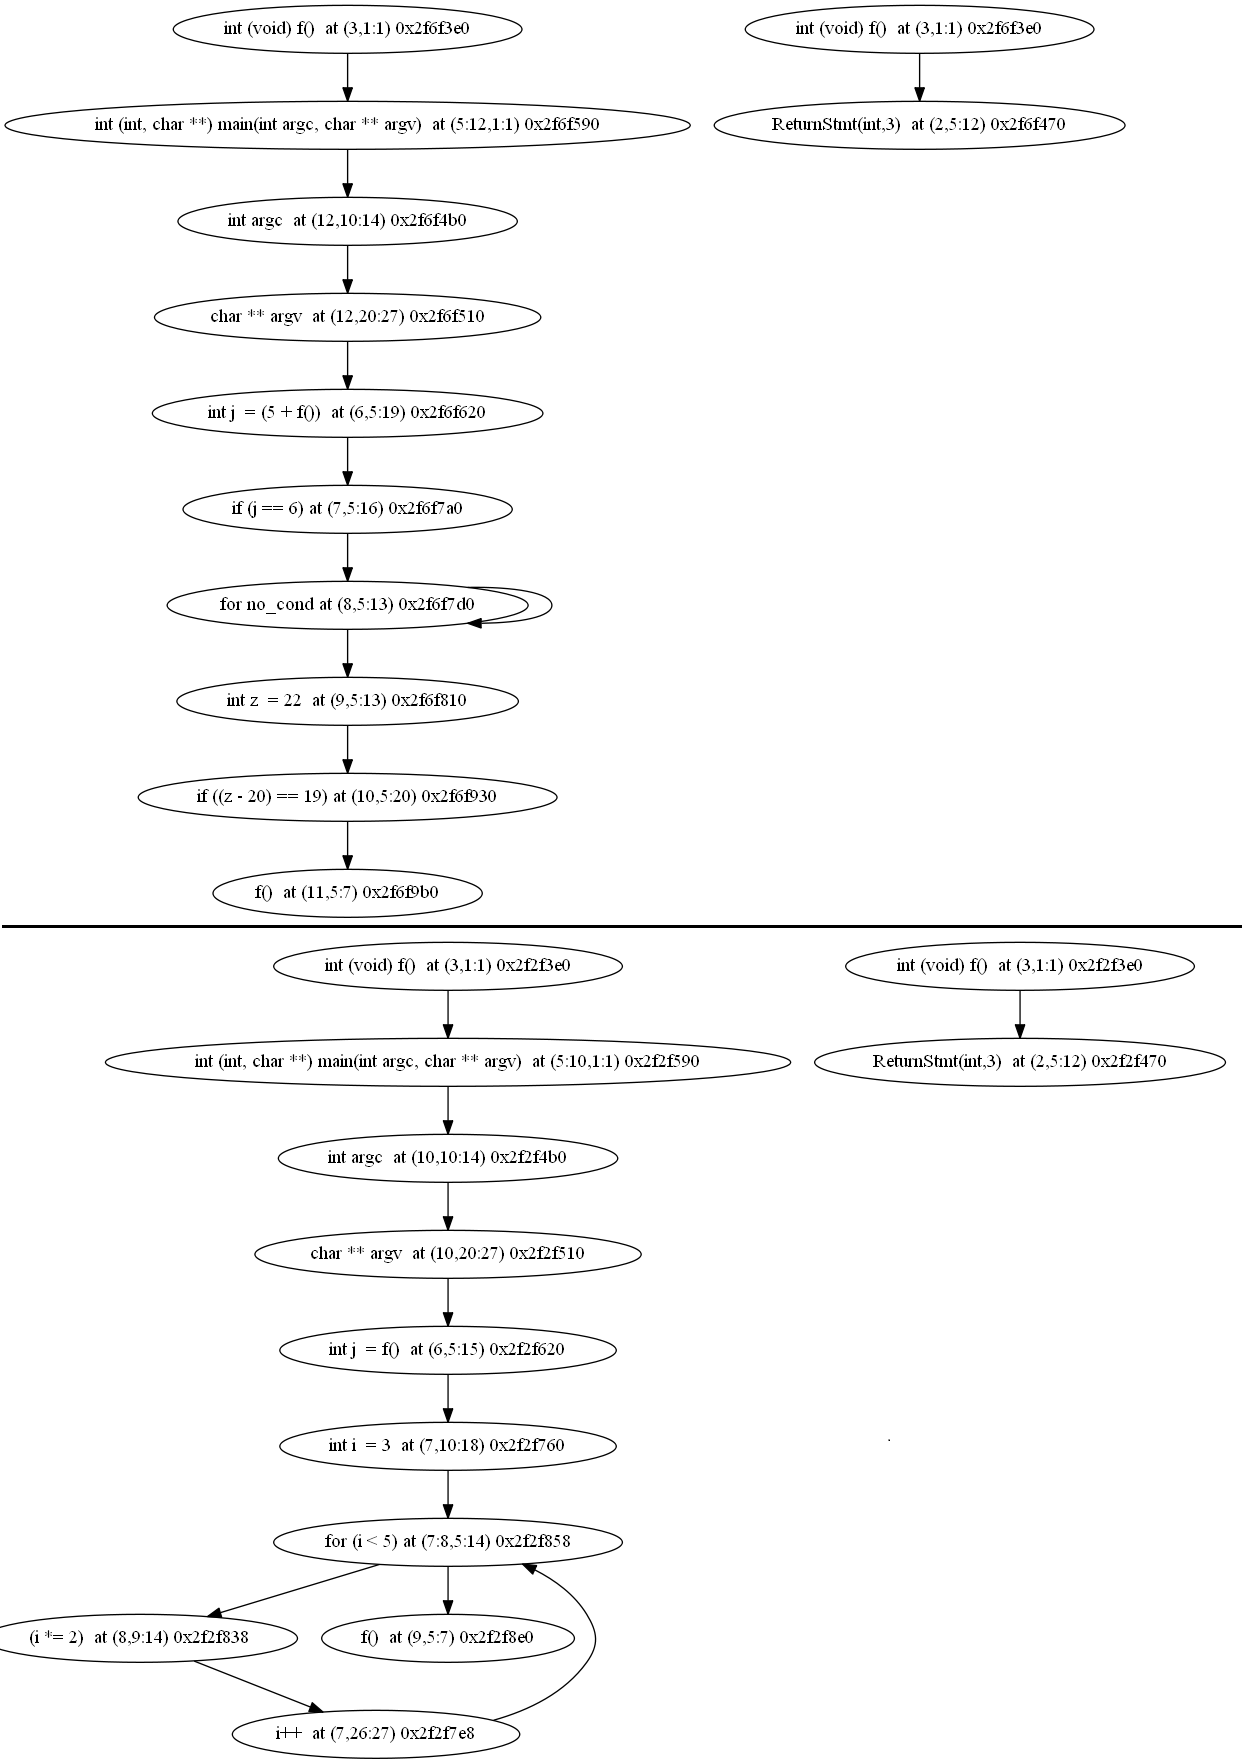
\includegraphics[scale=0.4]{data/for_example}
~\\~\\Figure I.3 - On the top, the output obtained for the example 1, on the bottom, for the example 5
\end{center}

\chapter{Testing the model checking algorithm}

\paragraph{}
\hspace{4mm}\textnormal{Unlike the CFG part, there is a lot of room here for automated tests because there are many elementary operations that must return a specific result. We have written some generic methods 
that enable to automatically check the output rather than performing a manual check. This constitutes a very simple 
testing framework that we will present here. We will then present our process and results for the first iteration.}

\section{Automated testing}

\paragraph{}
\hspace{4mm}\textnormal{All the test functions rely on generic methods such as \textbf{assertEquals} or \textbf{assertTrue} that print
the result of the test with its number. This way, it is fairly easy to generate a log file and get the result of the tests
in the clearest way. You can find below an example of such test functions :}

\begin{lstlisting}[language=scala]
def printMsg(failed: Boolean) = { 
        val msg = "\tTest %d %s".format(i,if (failed) "failed" else "passed") 
        if (failed) Console.err.println(msg)
        else        println(msg)
        i += 1
}
def assertEquals[T](t0: T, t1: T) = printMsg(t0 != t1)
def assertTrue(b: Boolean)       = printMsg(!b)
def compareEnv[T](envT1: Env[T], envT2: Env[T], expected: Env[T]) = assertEquals(envT1 interEnv envT2,    def testNeg[T](env: Env[T], envs: Env[T]*)  = assertEquals(!env,Set(envs: _*))
\end{lstlisting}
\section{Testing process}

\paragraph{}
\hspace{4mm}\textnormal{For this part, we have made a lot of unitary tests. We first tested every operation defined on the Environment subclasses
because it constitutes the base of almost all computations performed by the algorithm. Once we were assured that these operations were correctly implemented,
we tested the operations of the ModelChecker, starting with the elementary operations to the compound operations. 
After each modification, we ran the whole test as it has a reasonable exection times (less than a second).}

\begin{center}
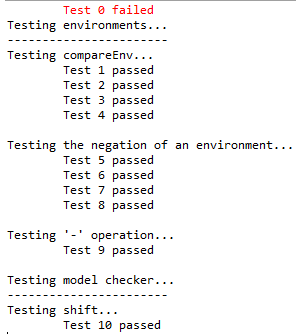
\includegraphics[scale=0.7]{data/test-log}
~\\~\\Figure II.1 - An example of a test log generated by our automatic tests
\end{center}

\paragraph{}
\hspace{4mm}\textnormal{We then wrote more advanced tests on small examples of graphs unrelated to any C++ code : just a few nodes and link to detect and fix obvious mistakes.
Finally, we tested the model checker against the CFG. Conveniently, the CFG conversion was already completely implemented when we starting to test the
model checker on C++ source codes. For this last testing step, we have had to manually check the output. Nevertheless, the test program was well-done and
easy-to-use. As the model checking algorithm takes some time to execute (a few seconds for a complicated property), it would have been unreasonable to execute the whole
tests, which processes many properties on different input codes (which have to be converted to CFG first). Therefore, we intensively used lazy values so that we can
test only the few properties we are interested in while having all the test cases defined in a single file.
The following snippet illustrates this strategy :}

\begin{lstlisting}[language=scala]
// when executed, it calls the Clang API on hidden_var_def.cpp, parses the AST file, convert it into a CFG,
// and generate a dot graph to help visualizing
lazy val checker1 = loadChecker("hidden_var_def")
lazy val test1 = {
	println("Testing the HIDDEN_VAR_DEF property...")
	printTest("Following lines are variable definitions that are hidden later in the code (may contain false positive results) :",
			checker1,HIDDEN_VAR_DEF)
}
	
lazy val checker2 = loadChecker("arith_pointer")
lazy val test2 = {
	println("Testing the ARITHMETIC_POINTER property...")
	printTest("Following lines contain an arithmetic expression involving a pointer :",checker2,ARITHMETIC_POINTER)
}

lazy val checker6 = loadChecker("unused_var")
lazy val test3 = {
       println("Testing the UNUSED_DECALRED_VAR property...")
       printTest("Following lines contain variable definition that are not used :",checker3,UNUSED_DECALRED_VAR)
}
// only test 1 is executed
test1
\end{lstlisting}
\paragraph{}
\hspace{4mm}\textnormal{The output is printed in the following form :}

\begin{center}
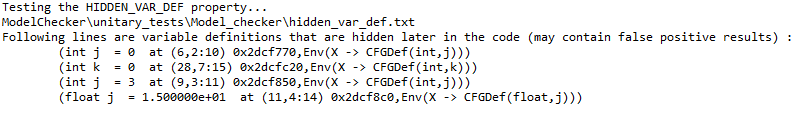
\includegraphics[scale=0.8]{data/test-log2}
~\\~\\Figure II.2 - Log file for the model checker testing program
\end{center}

\paragraph{}
\hspace{4mm}\textnormal{The properties we used for our tests were inspired from the MISRAC++ (a set of rules of good and bad practices) :}

\vspace{3mm}
\begin{itemize}
\item << There should not be function calls returning a value which is never used nor stored >>\vspace{1mm}
\item << There should not be hidden declarations in the code >>\vspace{1mm}
\item << There should not be arithmetic operations on pointer types other than the unary increment and decrement >>\vspace{1mm}
\item << There should not be declarations that are never used in any computation of any execution path >>\vspace{1mm}
\item ...\vspace{1mm}
\end{itemize}

\paragraph{}
\hspace{4mm}\textnormal{To each property corresponds a C++ input file. Below are the files corresponding to the two first properties.}

\begin{lstlisting}[language=java]
/**
 * UNUSED_FUNCTION_VALUE
 */
int f(int a, int b){
	return 1;
}

void g() { }

void h(int a) {
	a = 0;
}

float fun() {
	return 1.0f;
}

int main(int argc, char** argv) {
	g();
	int i = f(5,6) + 3;
 	// should return this line
	f(3,4);
	if (fun()) i = 0;
	// should return this line
	else       fun();
	while (f(5,fun())) {
		// should return this line
		f(1,6) + 1;
		// should return this line, with the right column (pointing at 5*(i - 9*fun()))
		if (f(4,2) + fun()) 5*(i - 9*fun());
	}
	return 0;
}

/**
 * HIDDEN_VAR_DEF
 */
int f(int q) {
    return q+2;
}

int main(int argc, char** argv) {
	int j = 0, q = 2;

	{
		// should return this line
		int j = 3;
		{
			// should not return this line (we are checking declarations of the same type)
			float j = 15.0f;
			{
				// should return this line
				float j;
				{
					// should not return this line (but it will, as a false positive result)
					int j = 18;
				}
			}
		}
	}
    if (j == 2)
    	f(q);

    if (false){
    	q = 7;
    }
    else {
    	while (true) {
    		int k = 0;
    	}
    }

    // should not return this line (but it will, as a false positive result)
    int k;
    return 0;
}
\end{lstlisting}
\end{document}
